% this file is called up by thesis.tex
% content in this file will be fed into the main document

%: ----------------------- name of chapter  -------------------------
%: ----------------------- paths to graphics ------------------------

% change according to folder and file names
\ifpdf
    \graphicspath{{5/figures/PNG/}{5/figures/PDF/}{5/figures/}}
\else
    \graphicspath{{5/figures/EPS/}{5/figures/}}
\fi

%: ----------------------- contents from here ------------------------

\captionsetup[subfigure]{labelfont=bf,textfont=normalfont,singlelinecheck=off,justification=centering}

\chapter{Evaluation of our algorithm in comparison to related algorithms} % top level followed by section, subsection
\section{Comparison to online SVM training algorithms: Pegasos and NORMA}
\label{ExperimentsNorma}
We compare our algorithm to both Pegasos \cite{Pegasos} and Norma \cite{Norma}, implemented on MATLAB for both the linear and the kernel-based case. The experiments are being run on AMD Phenom X4 965, with only one core being used for calculations. We perform several experiments, aiming to compare generalization error and convergence rates over different datasets, as well as the ability of the algorithm to adapt to the distribution with the changing parameters (flexibility and robustness) . 

We use several artificial datasets with known distributions and separation properties, and a Forest Covertype dataset (separating class 5 from other classes), originally used in \cite{Forest}, and also used for comparison of convergence speed in \cite{Pegasos}. The artificial datasets are generated  according to the following distributions:

\begin{enumerate}
  \item \emph{High-dimensional linearly separable data (Linear)} \label{it1} A random hyperplane is created in 50-dimensional space. Data points are generated randomly to both positive and negative sides of the hyperplane. Data points too close to the hyperplane are filtered out to create a clear margin. 
  \item \emph{High-dimensional linearly separable data with noise (Linear + noise)} Same as \ref{it1}, but 10\% of the labels are switched, simulating salt-and-pepper noise.
  \item \emph{Bayes-separable data (Bayesian)} \label{it3} This dataset is generated as described in \cite{Norma}, i.e. in such a way so that data is clearly separable using ideal Bayesian classifier for known class distributions.
  \item \emph{Bayes-separable data with moving distribution (Drifting)} As in \ref{it3}, but the parameters of a distribution are changed slightly each iteration, simulating target movement. This experiment estimates  the ability of the algorithms to adapt to gradual changes in the data distribution.
  \item \emph{Bayes-separable data with switching distribution (Switching)} Once again, a dataset generated according to the description in \cite{Norma}, with the distribution changed drastically every 1000 iterations. This experiment shows the ability of the algorithms to completely relearn a distribution. 
\end{enumerate}

For each distribution we measure the decrease of estimated error rate over training dataset (estimated error being simply the running average of the number of misclassified training samples divided by number of iterations in the averaging window), and the resulting error rate over the testing dataset (generated without noise in case of noisy distribution). In case of the dataset with the changing distribution, the distribution at the last iteration is used for testing.

For all experiments, the parameters of our algorithm were fixed, with $\lambda=0.02$, $\lambda_H=0.03$ and the cutoff parameter $r=150$. Pegasos and Norma used parameter $\lambda=0.02$, and either a linear kernel or a Gaussian RBF kernel with $\gamma=0.01$, which is the same value of $\gamma$ used for generating Bayes - separable datasets, which makes the resulting kernel an ideal case for separation.
\subsection{Experimental results}
The graphs for the estimated error rate are shown on figure \ref{Result:LinearPN} for linear implementation of NORMA and Pegasos, and on figure \ref{Result:GaussPN} for the kernel implementation, while the resulting error rate on the test datasets is shown in Table \ref{GenError}.
It can be  seen, that for linearly separable problems our algorithms performs on par with the Pegagos algorithm, with slight increase of the error rate possibly due to the overfitting. For kernel-based methods, however our algorithm usually outperforms both Norma and Pegasos, unless the exact kernel parameters are used, and even then (see Fig. \ref{Result:GaussPN}) our algorithm performs slightly better in the long run. It is interesting to note, that for switching dataset, NORMA actually outperforms Pegasos by a considerable margin, indicating that Pegasos algorithm is more sensitive to rapid changes in the classification target, most likely due to the rapid decay of the learning rate with time, while our algorithm was largely able to compensate, demonstrating stability of the method to condition changes. 

For the Covertype dataset, linear classifiers work best, and approach the error rates indicated in the paper(\cite{Forest}), with Pegasos and our algorithm giving virtually the same results. 

It is also important to note that, when compared to kernel-based SVM algorithms, our algorithm is much more efficient both in terms of computing and storage requirements, since the amount of weak classifiers, each requiring only a single inner product calculation, is much lower than the amount of kernel expansion terms produced by both NORMA and Pegasos for the same accuracy levels. For example, in the test shown on fig. \ref{Result:GaussPN} \subref{MG},  the resulting amount of kernel expansion terms was over 5000 after 10000 iterations (for both Norma and Pegasos), while the amount of weak classifiers generated by our method was only 67, i.e, both the memory and computational requirements (per classification) were less by a factor of around 75. 

\begin{figure*}[t]
    \centering
\begin{subfigure}[b]{.45\linewidth}
       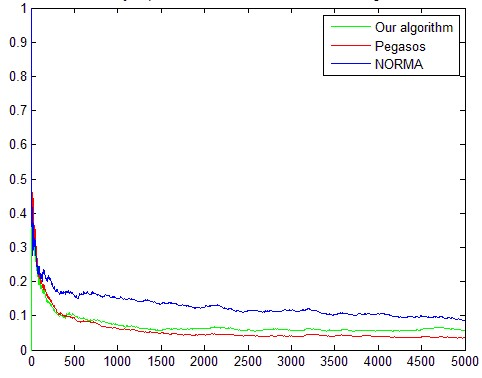
\includegraphics[width=0.9\linewidth]{PN_Lin_Lin}
\label{LL}
        \caption{Linearly separable dataset}
      \end{subfigure}%
\hspace{.01\linewidth}
\begin{subfigure}[b]{.45\linewidth}
	 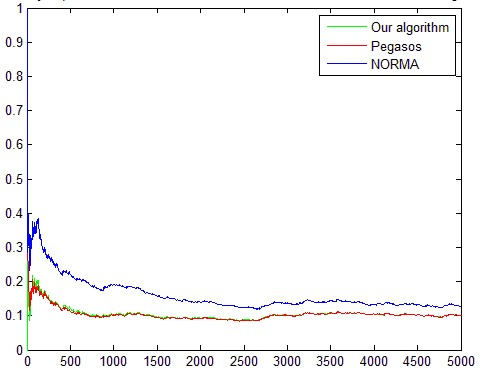
\includegraphics[width=0.9\linewidth]{PN_Noise_Lin.jpg}
       \label{NL}
      \caption{Linear dataset with noise}
  
	 \end{subfigure}%

 \begin{subfigure}[c]{.45\linewidth}
	   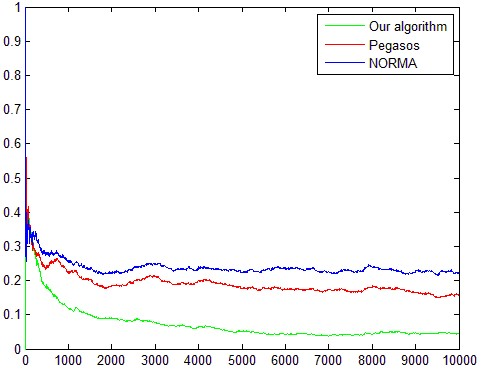
\includegraphics[width=0.9\linewidth]{PN_Bayess_Lin}
           \label{BL}
           \caption{Bayes-separable dataset with fixed distribution parameters}
 \end{subfigure}%
\hspace{.01\linewidth}
\begin{subfigure}[c]{.45\linewidth}
    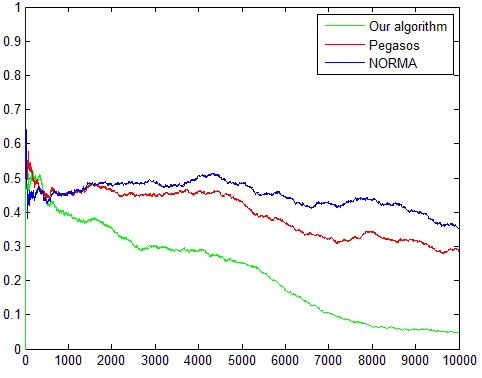
\includegraphics[width=0.9\linewidth]{PN_Move_Lin}
    \label{ML} 
   \caption{Bayes-separable dataset with drifting distribution parameters}
\end{subfigure}%

\begin{subfigure}[c]{.45\linewidth}
	   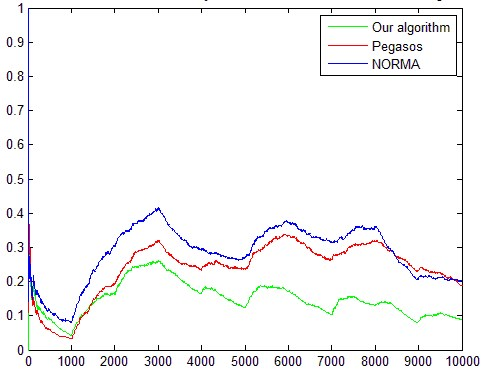
\includegraphics[width=0.9\linewidth]{PN_Switch_Lin}
\label{SL}
\caption{Bayes-separable dataset with parameters being switched every 1000 iterations}
\end{subfigure}%
\hspace{.01\linewidth}
\begin{subfigure}[c]{.45\linewidth}
	   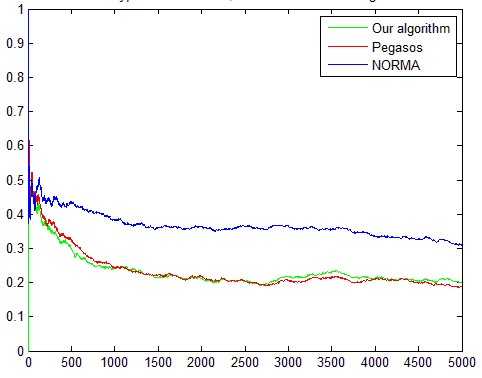
\includegraphics[width=0.9\linewidth]{PN_Cov_Lin}
\label{CtL}
\caption{ Covertype dataset}
\end{subfigure}%
    \caption{Experimental results comparing the performance of our algorithm to linear implementation of Pegasos and NORMA}
    \label{Result:LinearPN}
\end{figure*}

\begin{figure*}[t]
    \centering
\begin{subfigure}[b]{.45\linewidth}
       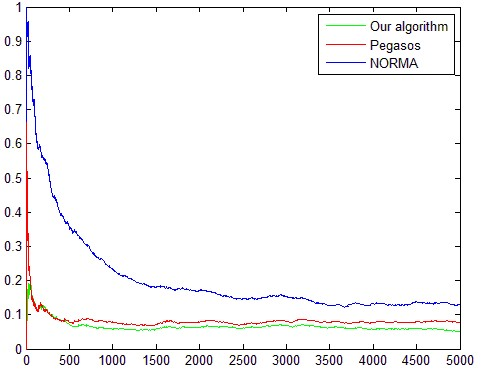
\includegraphics[width=0.9\linewidth]{PN_Lin_Gauss}
\label{LG}
        \caption{Linearly separable dataset}
      \end{subfigure}%
\hspace{.01\linewidth}
\begin{subfigure}[b]{.45\linewidth}
	 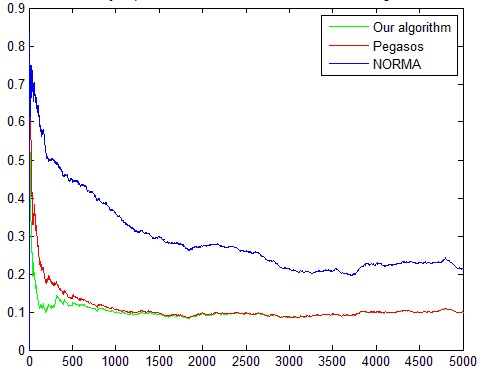
\includegraphics[width=0.9\linewidth]{PN_Noise_Gauss.jpg}
       \label{NG}
      \caption{Linear dataset with noise}
  
	 \end{subfigure}%

 \begin{subfigure}[c]{.45\linewidth}
	   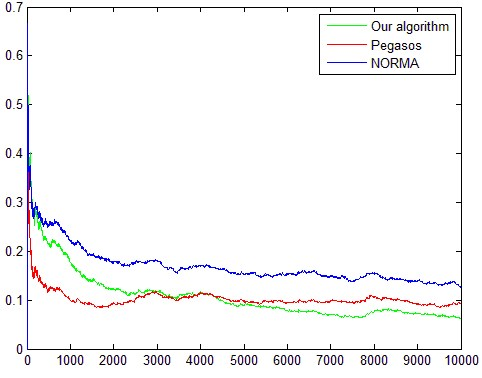
\includegraphics[width=0.9\linewidth]{PN_Bayess_Gauss}
           \label{BG}
           \caption{Bayes-separable dataset with fixed distribution parameters}
 \end{subfigure}%
\hspace{.01\linewidth}
\begin{subfigure}[c]{.45\linewidth}
    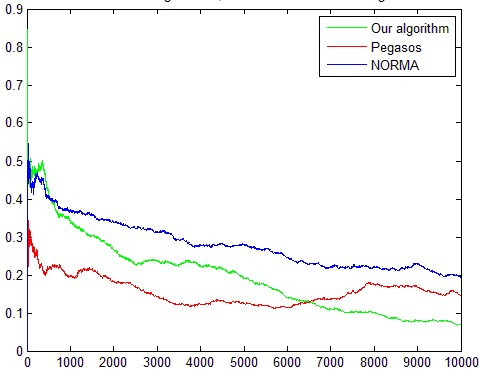
\includegraphics[width=0.9\linewidth]{PN_Move_Gauss}
    \label{MG} 
   \caption{Bayes-separable dataset with drifting distribution parameters}
\end{subfigure}%

\begin{subfigure}[c]{.45\linewidth}
	   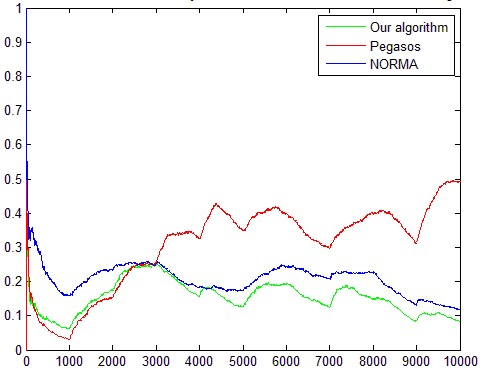
\includegraphics[width=0.9\linewidth]{PN_Switch_Gauss}
\label{SG}
\caption{Bayes-separable dataset with parameters being switched every 1000 iterations}
\end{subfigure}%
\hspace{.01\linewidth}
\begin{subfigure}[c]{.45\linewidth}
	   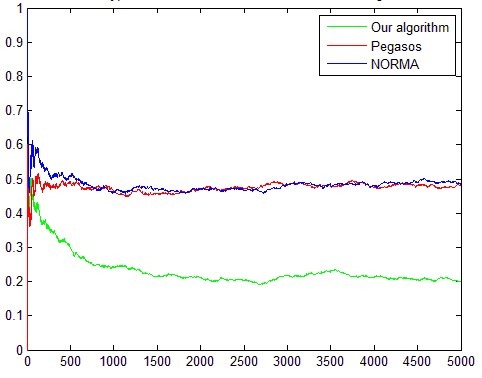
\includegraphics[width=0.9\linewidth]{PN_Cov_Gauss}
\label{CtG}
\caption{ Covertype dataset}
\end{subfigure}%
    \caption{Experimental results comparing the performance of our algorithm implementation of Pegasos and NORMA using Gaussian RBF}
    \label{Result:GaussPN}
\end{figure*}
\begin{table}
\centering
\begin{tabular}{| p{1.5cm}|  c |  c | c | c | c |}
\hline
 Dataset & O & PL & NL & PG & NG \\ \hline
Linear& 0.04 & 0.03 & 0.09 &0.07 &0.1 \\ \hline
Linear+ noise & 0.02 & 0.002 & 0.005 & 0.02 & 0.08 \\ \hline
Bayesian & 0.03 &0.17 & 0.22 & 0.08 & 0.15 \\ \hline
Drifting & 0.04 & 0.28 & 0.35 & 0.15&0.18 \\ \hline
Switching & 0.11 & 0.20 &0.21 & 0.32 & 0.13  \\ \hline
Covertype & 0.19 & 0.2 & 0.35 & 0.43 & 0.48 \\
\hline
\end{tabular}

\caption[Comparison to NORMA and Pegasos: Error rate over testing dataset]{Error rate over the testing dataset, O - our algorithm, PL -linear Pegasos, NL - linear NORMA, PG - Pegasos using Gaussian RBF kernel with $\gamma=0.01$, NG - NORMA with the same kernel}
\label{GenError}
\end{table}

\section{Comparison to offline algorithm: AdaBoost}
\label{AdaCompare}
In the interests of fairness, we also compare our algorithm to the AdaBoost in the offline setting. Since our algorithm is designed for online usage, we simulate the online environment by sequentially feeding it data samples randomly selected from the training dataset. Since a single iteration of the AdaBoost results in an additional weak classifier being added, while our algorithm takes $r$ iterations to do the same, to obtain equivalent conditions for testing we only evaluate the accuracy of our algorithm every $r$'s iteration. Also for equivalence, we use a pool of $M$ randomly selected linear classifiers for weak classifier selection.

It should be noted that the above condition does not mean that our algorithm is more computationally intensive, since to choose a classifier for addition the AdaBoost algorithm has to calculate weighted error rates of every classifier in the selection pool to select a maximum, or use some optimization algorithm to obtain best classifier in the case of continuous classifier pool, resulting, in the discrete case, in $MN$ classifier evaluations, where $N$ is the number of training samples. Our algorithm, however, only performs $rK$ evaluations,  with $r \ll N$ and $K$ being the number of classifiers already added.  In fact,  in the online case our algorithm is similar to AdaBoost evaluating on the random subset of the classifier pool on the random subset of training data. 
\begin{figure*}[t]
    \centering
\begin{subfigure}[b]{.45\linewidth}
       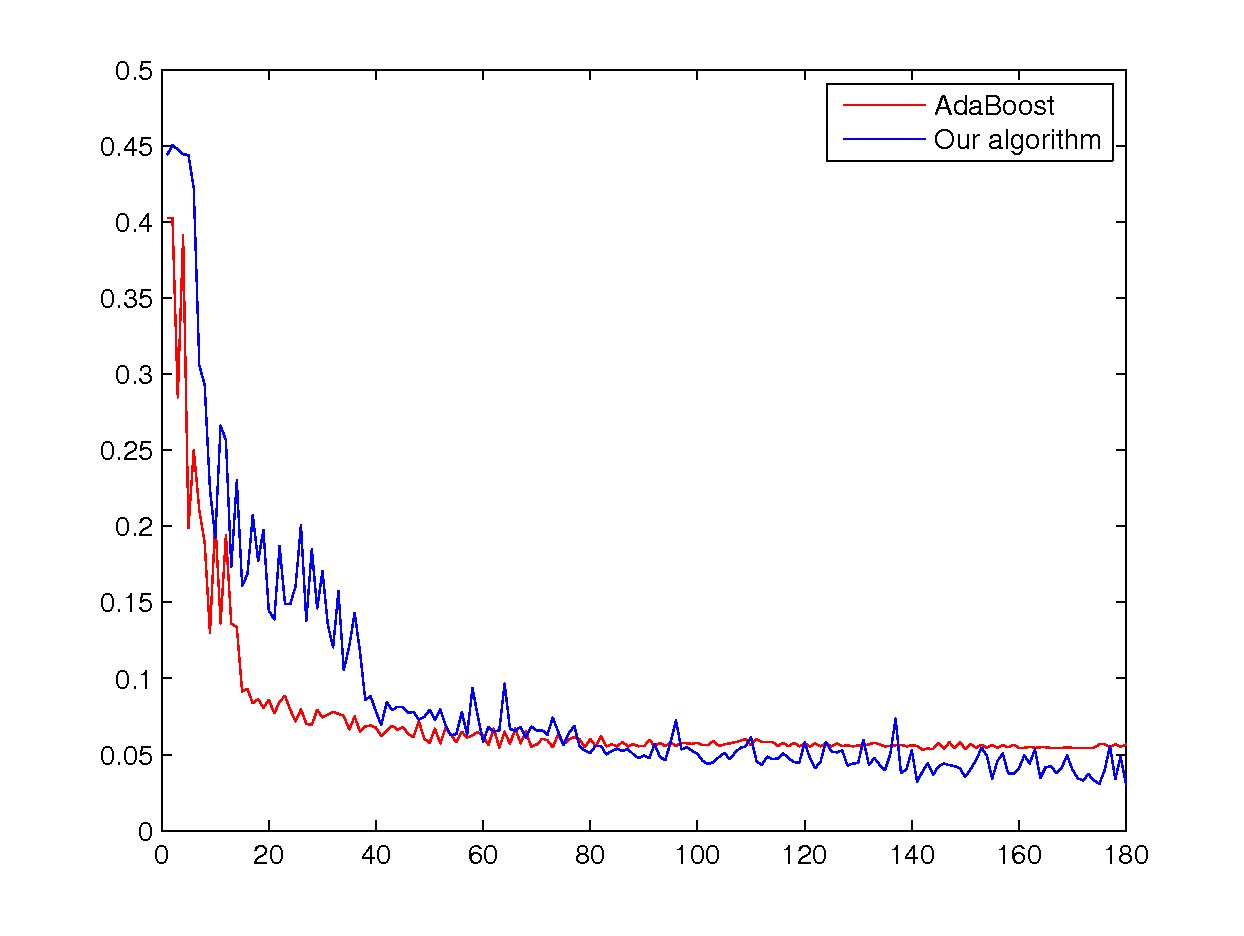
\includegraphics[width=0.9\linewidth]{adas}
\label{noref1}
        \caption{Synthetic nonlinear dataset}
      \end{subfigure}%
\hspace{.01\linewidth}
\begin{subfigure}[b]{.45\linewidth}
	 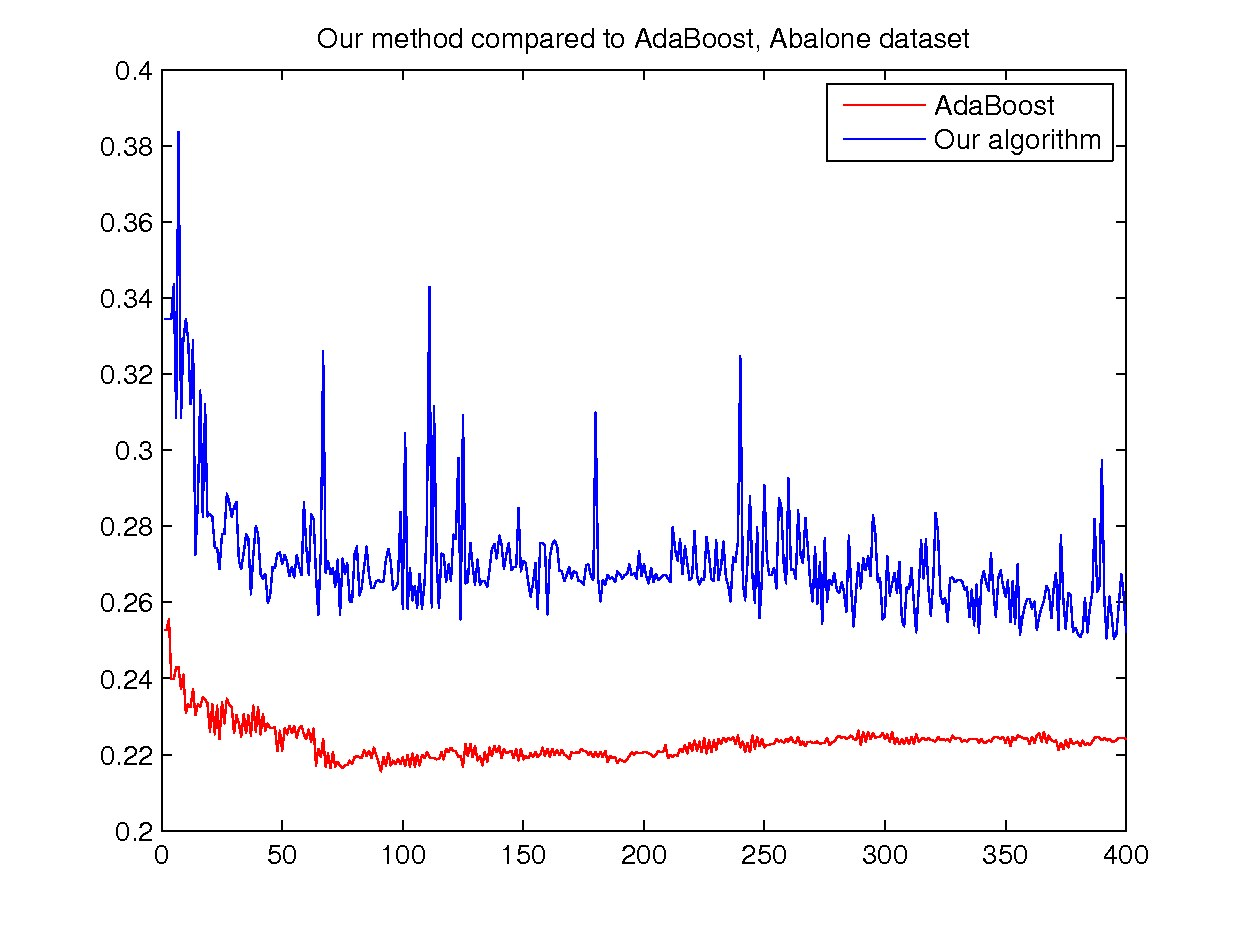
\includegraphics[width=0.9\linewidth]{adaab}
       \label{noref2}
      \caption{Abalone dataset}
  
	 \end{subfigure}%

    \caption{Experimental results comparing the performance of our algorithm to AdaBoost}
    \label{adacom}
\end{figure*}
We evaluate the methods on two datasets, one being a synthetic nonlinearly separable dataset, and the other  being the Abalone dataset from the UCI database (\cite{frafra}), with classes 10-29 merged into a positive class and other classes being negative. The results of generalized error on the number of classifiers added are presented on \figref{adacom}. They clearly show, that while on the offline setting AdaBoost outperforms our algorithm, the increase in the convergence speed is not very large. This advantage is due to the fact that our algorithm only selects near-optimal classifier on each addition, while AdaBoost uses the optimally selected one. 
\section{Comparison to the online AdaBoost}
\begin{figure}[t]
		\centering
		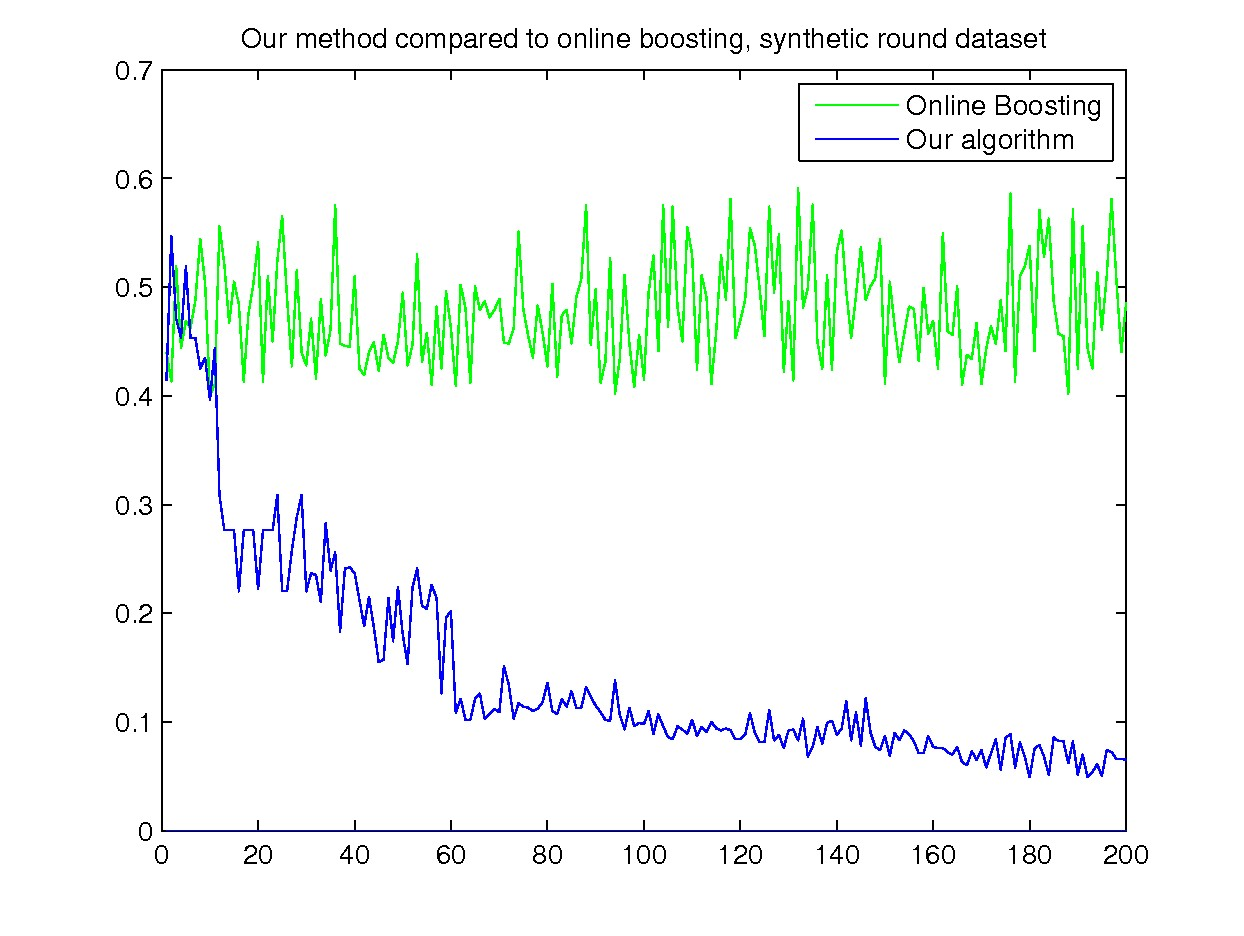
\includegraphics[width=0.7\textwidth]{odas}
		\caption{Experimental results comparing the performance of our algorithm to online boosting}
		\label{odacom}
	\end{figure}

We also compare our algorithm to the performance of the online AdaBoost presented in \cite{OnlineBoost}. We use the same datasets as in above section(\ref{AdaCompare}), with the difference being that the synthetic dataset is not pregenerated, since both of the algorithms are adapted to the online usage. 

For weak classifiers, we again use randomly generated linear classifiers, and for update stage of online Boosting algorithm we use the Pegasos iteration. 

The results of convergence experiments are shown on \figref{odacom}. They show that the online boosting algorithm underperforms compared to our algorithm, and is less stable. It does not converge well for both synthetic and Abalone dataset (not pictured).
It is also much more computationally expensive for the number of selectors equal to the number of classifiers added by our algorithm due to the fact that it performs updates on the whole pool of classifiers at once to estimate the optimal one. We can conclude that for most cases our algorithm would be superior to the online boosting.



% ---------------------------------------------------------------------------
%: ----------------------- end of thesis sub-document ------------------------
% ---------------------------------------------------------------------------

